\begin{figure}[t]
\begin{center}
\begin{subfigure}[b]{0.82\columnwidth}
  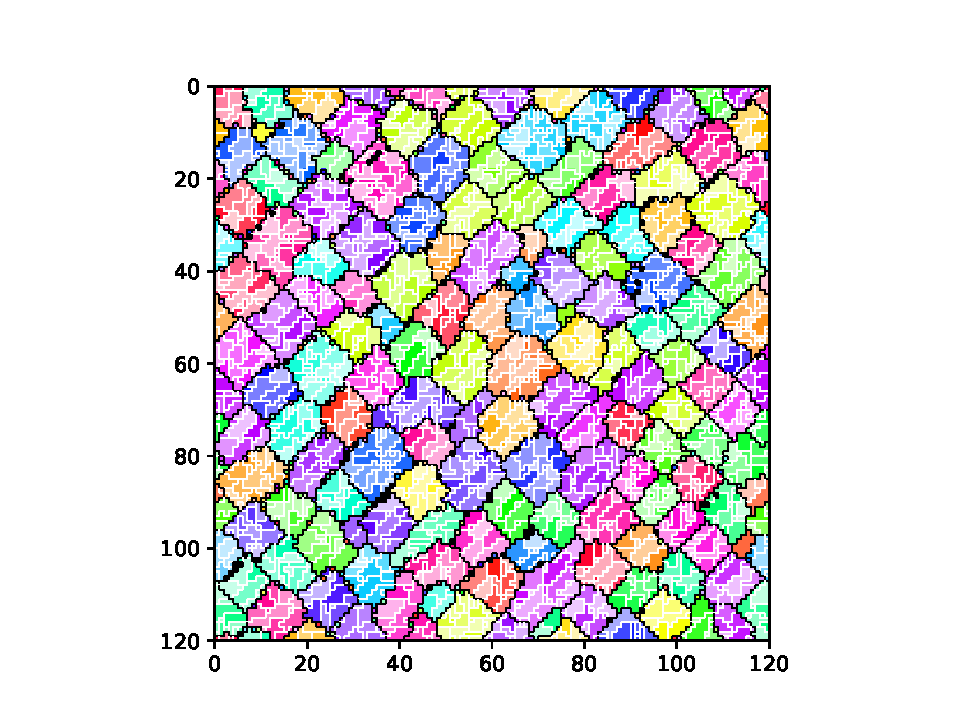
\includegraphics[width=\columnwidth,trim={2.5cm 0.5cm 2.5cm 1cm},clip]{img/ChannelMap_1022_update19500000}
  \caption{Mean $P_0 = 0.77$, $P_1 = 0.089$, $P_2 = 0.14$}
  \label{fig:ChannelMap_1022}
\end{subfigure}

\begin{subfigure}[b]{0.82\columnwidth}
  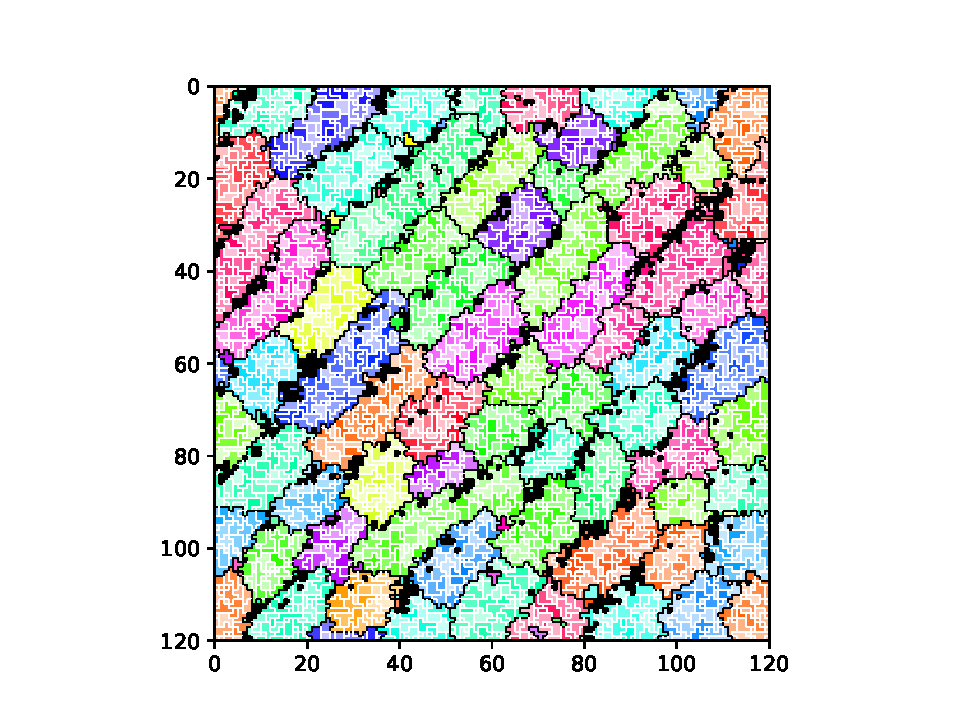
\includegraphics[width=\columnwidth,trim={2.5cm 0.5cm 2.5cm 1cm},clip]{img/ChannelMap_1041_update19500000}
  \caption{Mean $P_1 = 1.0$}
  \label{fig:ChannelMap_1041}
\end{subfigure}

\begin{subfigure}[b]{0.82\columnwidth}
  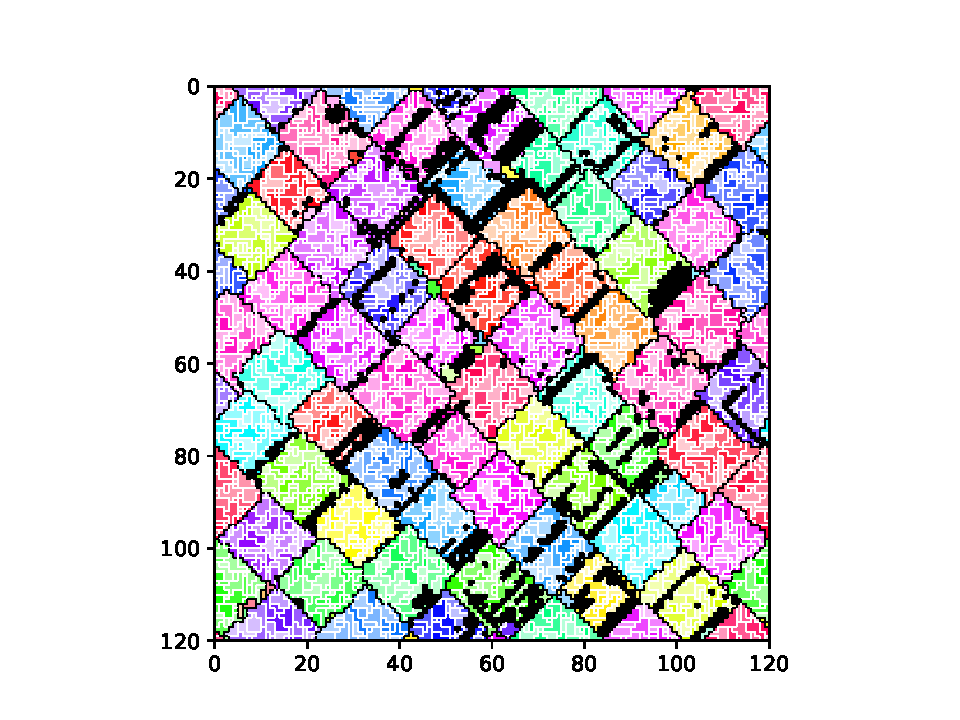
\includegraphics[width=\columnwidth,trim={2.5cm 0.5cm 2.5cm 1cm},clip]{img/ChannelMap_1008_update19500000}
  \caption{Mean $P_2 = 1.0$}
  \label{fig:ChannelMap_1008}
\end{subfigure}

\caption{
State of same-channel zero- and one-level signaling networks after $1.95 \times 10^{10}$ updates of evolution with different population mean $P_0$, $P_1$, and $P_2$.
Zero-level channels coded by HSV value are separated by white borders and one-level channels coded by HSV hue are separated by black borders.
}
\label{fig:outcome_grids}
\end{center}
\end{figure}
